
Como lo indica el título de esta sección, en este primer experimento se determinará la impedancia de salida del amplificador (con placa auxiliar) presentado en la sección de \textit{Materiales e Instrumentos}, en el apartado \ref{sec:Amp1}. 

Los fundamentos de este experimento se encuentran en la sección de \textit{Marco Teórico} en el apartado \ref{sec:Zi}.

\subsubsection{Implementación}

Para efectuar las mediciones que se requieren en este experimento, se conectó los instrumentos se muestra a continuación (figura \ref{fig:conexZoLA}).

\begin{figure}[H]
    \centering
    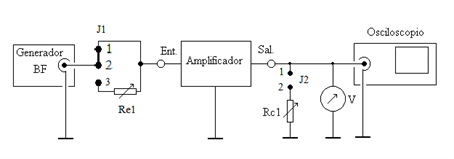
\includegraphics[width=0.9\textwidth]{Imagenes/conexZoLA.png}
    \caption{Conexión del Amplificador de prueba para medir la impedancia de salida}
    \label{fig:conexZoLA}
\end{figure}

El amplificador fue alimentado con una fuente de tensión de 12 V, y la señal de entrada (creada por el generador) tenía una frecuencia de 1 kHz.

Ahora el amplificador se encuentra sin resistencia de carga ($R_{C_1}$), por lo que la tensión que se medirá con el voltímetro y el osciloscopio, será la tensión de salida en vacío. Se procede a variar la tensión de entrada (del generador) hasta justo antes de que la señal de salida se vea recortada (antes de que el amplificador entre en la zona de funcionamiento alineal). Esto se realiza exclusivamente con la finalidad de lograr trabajar con señales más grande para que así sea mas fácil analizarlas y que se vean menos afectadas por el ruido.

La señal de salida $v_s$ máxima que se obtuvo sin recortes fue de 10,2 $V_{pp}$, con una señal de entrada $v_i$ = 3.08 $V_{pp}$.

Sabiendo la tensión de salida en vacío con esa tensión de entrada, se procedió a conectar la carga $R_{C_1}$ (resistor variable), con el jumper $J2$ y se fue variando la resistencia hasta obtener en la salida una señal con la mitad de la amplitud de la señal original. El valor más próximo a este que se obtuvo fue de $v_s'$ = 5,08 $V_{pp}$.

%imagen de la medicion

En esta situación el valor de la impedancia de salida del amplificador es numéricamente igual a la resistencia de carga (debido al tipo de amplificador y la frecuencia en que se hace el ensayo, se puede considerar sin mucho margen de error que la impedancia de salida no tiene parte reactiva considerable), y su valor puede determinarse en forma indirecta midiendo el valor de la resistencia de carga $R_{C_1}$ con un óhmetro. 

Por lo que sin alterar la resistencia, se desconectó el jumper $J2$ para que la medición no se viese afectada por el resto del circuito y se midió la resistencia $R_{C_1}$. En la tabla a continuación se exponen los datos de resistencia recogidos junto con la incertidumbre en la medición (tabla \ref{tab:exp1}).

\subsubsection{Mediciones}

Para la medición de la resistencia se utilizó el multímetro del laboratorio de la marca UNI-T, modelo UT890C, cuyos datos de exactitud, se encuentra en la sección \ref{sec:Información Instrumentos} (Información de Instrumentos), en la tabla \ref{tab:R_UT890C}.

\begin{table}[H]
    \centering
    \scalebox{1}{
    \begin{tabular} {|c|c|c|c|c|}
    %{|m{1.5cm}|m{2.7cm}|m{1cm}|p{1.5cm}|m{2.7cm}|}
   
    \hline
         $f$ & Valor Nominal & $V_s$ & $R_{C_1}=R_o$ & Incertidumbre \\
         
         Frec. Gen. & de $Z_{sal}=R_o$ & en vacío & Para $V_s'=\frac{V_s}{2}$ & medición $R_{C_1}$\\
    \hline
        1 kHz & 50 $\ohm$ & 10.2 $V_{pp}$ & 46.1 $\Omega$ & $\pm$ 0.869 $\Omega$\\
    \hline
        \end{tabular}}
        \def\tablename{Tabla} 
        \caption{Valores esperados y obtenidos}
        \label{tab:exp1}
\end{table}

Afortunadamente, el valor de resistencia obtenido, coincide bastante con el valor esperado para la resistencia de salida. Este es incluso menor, lo que representaría una característica positiva, ya que la impedancia de salida de un amplificador ideal debería ser cero.
